\section{Background}
The no rainbow problem is quite complex and can be understood in a lot of different ways.
To understand the problem as broadly as possible a few different areas of discrete mathematics are needed.

\subsection{Equivalence classes and equivalence relations}
Equivalence classes are used to group things that are equal in some sense.
This requires we have a set of objects and an binary operator we can use to check if they are equal.
In this general case we use $\sim$ as the operator.

$$
  a \sim b \implies \textit{$a$ is related to $b$ under the equivalence relation ($\sim$)}
$$

A common way of defining equivalence relations is to map the objects to their image and then use equality.
More generally we can define it using:
$$
  a \sim b \iff f(a) = f(b)
$$
Where $f(a)$ is the image of $a$.

For example:
$$
  a \sim b \iff (a \bmod 3) = (b \bmod 3) : \quad a, b \in \mathds{Z}
$$

Here we send each object to their image -- which is their remained after division by 3 -- and then compare them.
Here we get 3 equivalence classes $\{[0], [1], [2]\}$. All integers are mapped into exactly one of these 3 equivalence class.

The representative of a class is the element which has itself as image. In other words, $f(a) = a \iff a$ is a representative.
\cite[Section 7.3]{sourceArmen} \cite[Section 1.2]{sourceAATA}

\subsection{Graphs}
Graphs consist of a set of edges and a set of nodes.
Nodes are usually presented as circles with edges connecting the circles as lines, as presented in \ref{figGraphExample}.
Usually an edge is some kind of relationship. 
A graph is a very powerful and general tool for modeling many problems.

\begin{center}
\begin{figure}[h]
\centering
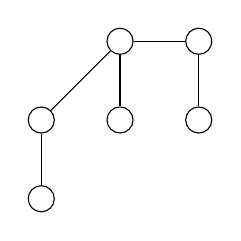
\begin{tikzpicture}[main/.style = {draw, circle}]
    \node[main] (A) {};
    \node[main] (B) [left of=A] {};
    \node[main] (C) [below of=A] {};
    \node[main] (D) [left of=C] {};
    \node[main] (E) [left of=D] {};
    \node[main] (F) [below of=E] {};

    \draw (A) -- (B);
    \draw (A) -- (C);
    \draw (B) -- (D);
    \draw (B) -- (E);
    \draw (F) -- (E);
\end{tikzpicture}
  \caption{An example of a graph.}
  \label{figGraphExample}
\end{figure}
\end{center}

\cite[Chapter 1]{sourceDiestel}
\cite[Chapter 1]{sourceGWA}
\cite[Section 9.1]{sourceArmen}

% Does this add anything?

\subsection{Hyper Graphs}
A hyper graph is similar to a normal graph.
But in a hyper graph edges connect multiple nodes, usually more than 2.
A hyper edge which is 2-regular is a "normal" graph.
The "normal" graph can be seen as a special case of the hyper graph.

Another way of phrasing it is that an edge is a set of nodes instead of a pair.

A hyper graph is the kind of graph the no rainbow problem is interesting for.

\begin{center}
\begin{figure}[h]
\centering
\begin{tikzpicture}[main/.style = {draw, circle}]
    \node[main] (a) at (0,2) {a};
    \node[main] (b) at (2,2) {b};
    \node[main] (c) at (4,2) {c};
    \node[main] (d) at (0,4) {d};
    \node[main] (e) at (2,4) {e};
    \node[main] (f) at (4,4) {f};

    \begin{scope}[fill opacity=0.5]
    \filldraw[fill=yellow!70] 
        plot [smooth cycle, tension=1.5]
        coordinates {
          ($(a)+(-0.8,0)$) 
          ($(b)+(0,0.8)$) 
          ($(c)+(0.8,0)$)
          ($(b)+(0,-0.8)$) 
        };

    \filldraw[fill=blue!70] 
        plot [smooth cycle, tension=0.8]
        coordinates {
          ($(c)+(0,-0.8)$) 
          ($(f)+(0.8,0.8)$) 
          ($(e)+(-0.4,0.4)$)
        };

    \filldraw[fill=red!70] 
        plot [smooth cycle, tension=1.5]
        coordinates {
          ($(d)+(-0.8,0)$) 
          ($(e)+(0,0.8)$) 
          ($(f)+(0.8,0)$)
          ($(e)+(0,-0.8)$) 
        };

    \filldraw[fill=green!70] 
        plot [smooth cycle, tension=1.0]
        coordinates {
          ($(c)+(-0.4,-0.4)$) 
          ($(c)+(0.4,0.4)$) 
          ($(e)+(0,0.8)$)
          ($(a)+(-0.4,0.4)$) 
          ($(a)+(0.4,-0.4)$) 
          ($(e)+(0,-0.8)$)
        };

    \end{scope};

    \node[main] (a) at (0,2) {a};
    \node[main] (b) at (2,2) {b};
    \node[main] (c) at (4,2) {c};
    \node[main] (d) at (0,4) {d};
    \node[main] (e) at (2,4) {e};
    \node[main] (f) at (4,4) {f};
\end{tikzpicture}
  \caption{An example of a hyper graph.}
  \label{figHyperGraphExample}
\end{figure}
\end{center}

% Show the other way of rendering them

The hyper graph shown in figure \ref{figHyperGraphExample} is $3$-regular.
A hyper graph is $r$-regular if and only if all edges connect $r$-different nodes.
\cite{sourceHyper}

\subsubsection{Node coloring as related by the no rainbow problem}
A node coloring is a mapping from nodes to colors.
There are usually constraints on what colors can be part of an edge.
The color of a node is denoted as $c(a)$, where $a$ is the node and $c$ is the coloring.
Since a coloring is a mapping it can be thought of as a function that takes you from a node to the color of the node.
A color is usually a letter or a number.

The constraints added in the no rainbow problem are
\begin{enumerate}
  \item No edge can have all r-colors -- no rainbow edges
  \item All colors have to be represented in the graph -- the coloring is surjective
\end{enumerate}

An example of a valid coloring in the no rainbow problem for the graph presented above is $c(d)=0, c(b)=1, c(*)=2$, where $*$ denotes all other nodes.
There are a lot more valid colorings, though this coloring is particularly simple.
The validity of a coloring is dictated by the edges added in the graph.
A multi graph with the maximum number of edges (called a complete graph) has no valid no-rainbow coloring.
A multi graph without any edges is trivial to find a no-rainbow coloring for.
The cases in between are the main topic of this thesis.

\cite{sourceHyper}
% Is a complete r-regular subgraph enough to disprove there is a no-rainbow coloring? 

\subsection{The existing algorithms}
TBA

\subsection{Algorithm basics}
TBA
